\section{Work definition and division}
\label{ch:wdd}
This chapter provides an overview of the work involved in the development of an inflatable guidable aeroshell and the allocation of human resources to the defined activities. It is essential that planning is adhered to in order to fulfill customer requirements within the allotted timeframe of ten weeks in total with the available resources, namely a team consisting of nine students. 

To this end a \gls{wbs} and \gls{wfd} are presented that categorize and sequence the work activities involved in the project in section \ref{sec:work}. Secondly, managerial and technical functions are appointed to team members in section \ref{sec:org}. Thirdly, the allocation of human resources in time is presented in the form of a Gantt chart in section \ref{sec:gantt}.

\subsection{Work definition}
\label{sec:work}
Work activities are recognized and categorized as depicted in Fig. \ref{fig:wbs}. The \gls{wbs} presented distinguishes conceptual design from preliminary design, where the former is conducted on five concepts and the latter on the concept selected in the trade-off made during the \acrfull{mtr}. This report details the activities taken up to the point of the trade-off, primarily the steps of development and implementation of tools and the analysis of concepts through analysis with the developed tools. Conceptual concept analysis and design takes place on a high level and is centered around the performance of the selected concepts in terms of the trade-off criteria. Preliminary analysis and design proceeds in more detail. Therefore tools are required that allow a more detailed analysis and design, captured by the work activities of tool set expansion. While it is preferable to have a more detailed analysis and design of all selected concepts, the allocated timeframe is a limiting factor. To maximize work efficiency within this timeframe, it is essential that a good planning is made and adhered to. This planning is discussed in section \ref{sec:gantt}.

The \gls{wfd}, presented in Fig. \ref{fig:wfd}, sequences the work activities defined. Primary goal of the \gls{wfd} is to depict how work activities interact, required for a time-constrained resource allocation, and to identify iteration loops.

\begin{sidewaysfigure}[ht]
    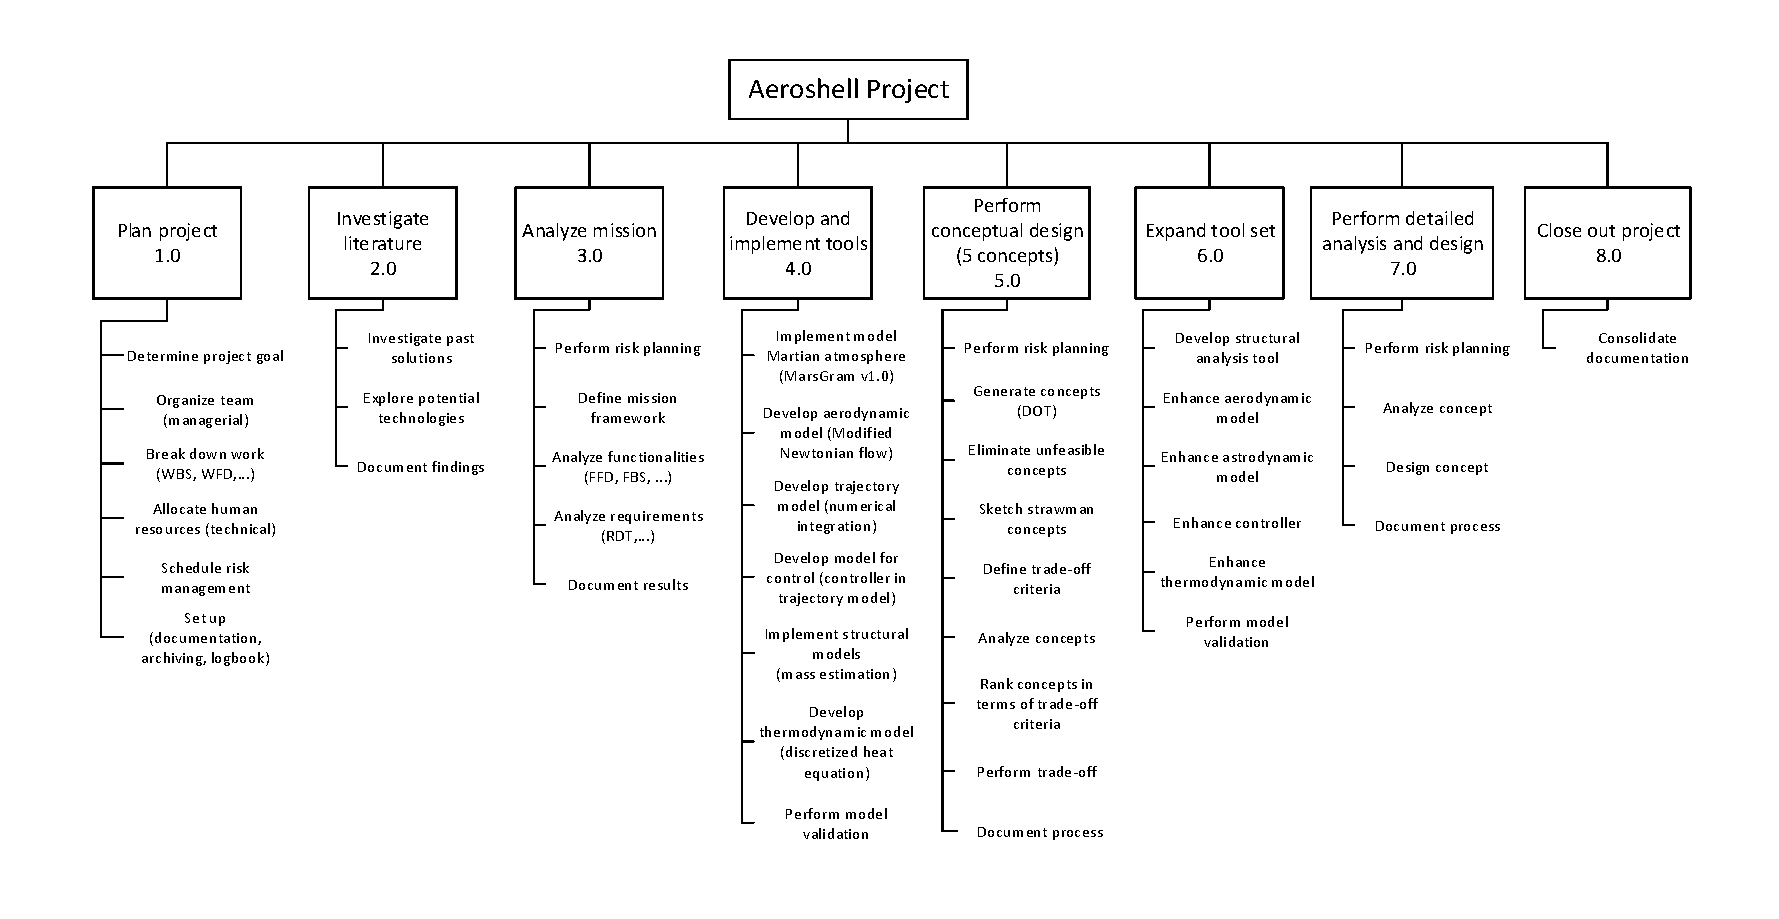
\includegraphics[scale=0.85]{Figure/WBS_MTR.pdf}
    \caption{\acrfull{wbs} of project}
    \label{fig:wbs}
\end{sidewaysfigure}
\begin{sidewaysfigure}[ht]
    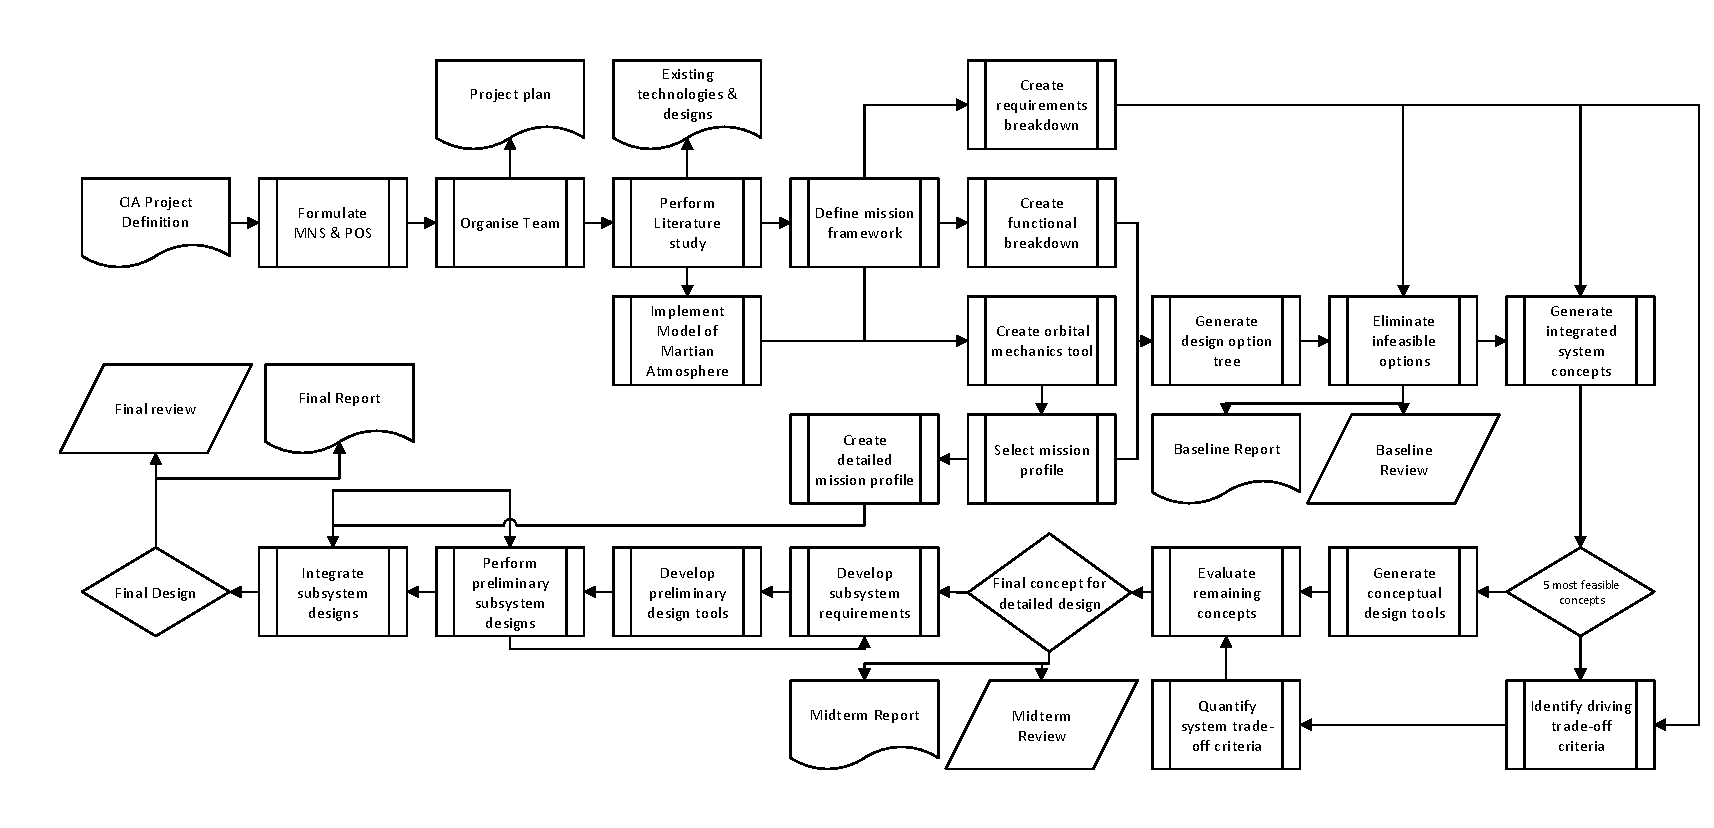
\includegraphics[scale=0.85]{Figure/WFD_MTR.pdf}
    \caption{\acrfull{wfd} of project}
    \label{fig:wfd}
\end{sidewaysfigure}

\subsection{Technical and managerial team organisation}
\label{sec:org}
Technical functions, as appointed in the \acrfull{pp} \cite{Balasooriyan2015}, have been maintained up to the \gls{mtr} and will be maintained hereafter. This is based on the reasoning that members have gained knowledge and experience of their respective appointed fields to such an extent that their primary responsibility should lie therein. All team members are involved in each field, however, by active communication and interaction during start-of-day, end-of-day and status meetings. The departments are: structural, aerodynamics, control systems $\&$ trajectory and thermodynamics. They are depicted in Fig. \ref{fig:obs}. Department descriptions have been taken up in Appendix \ref{app:obs}

Organisational functions are depicted in Fig. \ref{fig:obs}. The organisational functions will be re-divided amongst team members after the \gls{mtr}, in order to fully explore the capabilities of and to provide the best possible learning experience for all team members. The function descriptions have been taken up in Appendix \ref{app:obs}.

\begin{figure}[H]
\centering
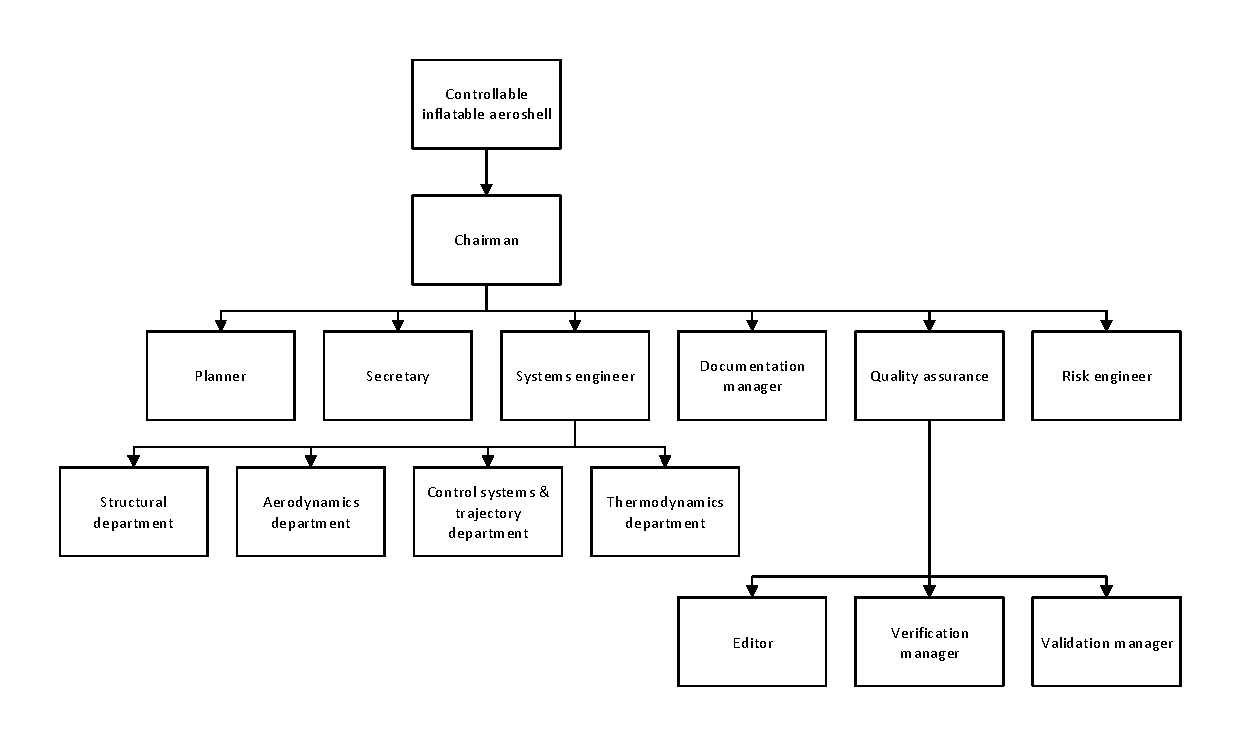
\includegraphics[width=0.95\textwidth]{./Figure/OBS_MTR.pdf}
\caption{Organisational breakdown structure} \label{fig:OBS}
\label{fig:obs}
\end{figure}

\subsection{Human resource allocation}
\label{sec:gantt}
The work activities have been defined in the \gls{wbs} displayed in Fig. \ref{fig:wbs} and sequenced in the \gls{wfd} in Fig. \ref{fig:wfd}. Human resources are allocated to these activities in the Gantt chart, presented in Appendix \ref{app:gantt}. The planner ensures that all team members work according to the deadlines defined in the Gantt chart. Actions taken in case of deadline exceedance are dependent on the nature of the delay.
